% Options for packages loaded elsewhere
\PassOptionsToPackage{unicode}{hyperref}
\PassOptionsToPackage{hyphens}{url}
\PassOptionsToPackage{dvipsnames,svgnames,x11names}{xcolor}
%
\documentclass[
  xelatex,
  ja=standard]{bxjsarticle}

\usepackage{amsmath,amssymb}
\usepackage{iftex}
\ifPDFTeX
  \usepackage[T1]{fontenc}
  \usepackage[utf8]{inputenc}
  \usepackage{textcomp} % provide euro and other symbols
\else % if luatex or xetex
  \usepackage{unicode-math}
  \defaultfontfeatures{Scale=MatchLowercase}
  \defaultfontfeatures[\rmfamily]{Ligatures=TeX,Scale=1}
\fi
\usepackage{lmodern}
\ifPDFTeX\else  
    % xetex/luatex font selection
  \setmainfont[BoldFont=Noto Sans CJK JP]{Noto Serif CJK JP}
\fi
% Use upquote if available, for straight quotes in verbatim environments
\IfFileExists{upquote.sty}{\usepackage{upquote}}{}
\IfFileExists{microtype.sty}{% use microtype if available
  \usepackage[]{microtype}
  \UseMicrotypeSet[protrusion]{basicmath} % disable protrusion for tt fonts
}{}
\makeatletter
\@ifundefined{KOMAClassName}{% if non-KOMA class
  \IfFileExists{parskip.sty}{%
    \usepackage{parskip}
  }{% else
    \setlength{\parindent}{0pt}
    \setlength{\parskip}{6pt plus 2pt minus 1pt}}
}{% if KOMA class
  \KOMAoptions{parskip=half}}
\makeatother
\usepackage{xcolor}
\setlength{\emergencystretch}{3em} % prevent overfull lines
\setcounter{secnumdepth}{5}
% Make \paragraph and \subparagraph free-standing
\ifx\paragraph\undefined\else
  \let\oldparagraph\paragraph
  \renewcommand{\paragraph}[1]{\oldparagraph{#1}\mbox{}}
\fi
\ifx\subparagraph\undefined\else
  \let\oldsubparagraph\subparagraph
  \renewcommand{\subparagraph}[1]{\oldsubparagraph{#1}\mbox{}}
\fi


\providecommand{\tightlist}{%
  \setlength{\itemsep}{0pt}\setlength{\parskip}{0pt}}\usepackage{longtable,booktabs,array}
\usepackage{calc} % for calculating minipage widths
% Correct order of tables after \paragraph or \subparagraph
\usepackage{etoolbox}
\makeatletter
\patchcmd\longtable{\par}{\if@noskipsec\mbox{}\fi\par}{}{}
\makeatother
% Allow footnotes in longtable head/foot
\IfFileExists{footnotehyper.sty}{\usepackage{footnotehyper}}{\usepackage{footnote}}
\makesavenoteenv{longtable}
\usepackage{graphicx}
\makeatletter
\def\maxwidth{\ifdim\Gin@nat@width>\linewidth\linewidth\else\Gin@nat@width\fi}
\def\maxheight{\ifdim\Gin@nat@height>\textheight\textheight\else\Gin@nat@height\fi}
\makeatother
% Scale images if necessary, so that they will not overflow the page
% margins by default, and it is still possible to overwrite the defaults
% using explicit options in \includegraphics[width, height, ...]{}
\setkeys{Gin}{width=\maxwidth,height=\maxheight,keepaspectratio}
% Set default figure placement to htbp
\makeatletter
\def\fps@figure{htbp}
\makeatother

\renewcommand{\thefootnote}{\arabic{footnote}}
\makeatletter
\makeatother
\makeatletter
\makeatother
\makeatletter
\@ifpackageloaded{caption}{}{\usepackage{caption}}
\AtBeginDocument{%
\ifdefined\contentsname
  \renewcommand*\contentsname{目次}
\else
  \newcommand\contentsname{目次}
\fi
\ifdefined\listfigurename
  \renewcommand*\listfigurename{図一覧}
\else
  \newcommand\listfigurename{図一覧}
\fi
\ifdefined\listtablename
  \renewcommand*\listtablename{表一覧}
\else
  \newcommand\listtablename{表一覧}
\fi
\ifdefined\figurename
  \renewcommand*\figurename{図}
\else
  \newcommand\figurename{図}
\fi
\ifdefined\tablename
  \renewcommand*\tablename{表}
\else
  \newcommand\tablename{表}
\fi
}
\@ifpackageloaded{float}{}{\usepackage{float}}
\floatstyle{ruled}
\@ifundefined{c@chapter}{\newfloat{codelisting}{h}{lop}}{\newfloat{codelisting}{h}{lop}[chapter]}
\floatname{codelisting}{コード}
\newcommand*\listoflistings{\listof{codelisting}{コード一覧}}
\makeatother
\makeatletter
\@ifpackageloaded{caption}{}{\usepackage{caption}}
\@ifpackageloaded{subcaption}{}{\usepackage{subcaption}}
\makeatother
\makeatletter
\@ifpackageloaded{tcolorbox}{}{\usepackage[skins,breakable]{tcolorbox}}
\makeatother
\makeatletter
\@ifundefined{shadecolor}{\definecolor{shadecolor}{rgb}{.97, .97, .97}}
\makeatother
\makeatletter
\makeatother
\makeatletter
\makeatother
\ifLuaTeX
\usepackage[bidi=basic]{babel}
\else
\usepackage[bidi=default]{babel}
\fi
\babelprovide[main,import]{japanese}
% get rid of language-specific shorthands (see #6817):
\let\LanguageShortHands\languageshorthands
\def\languageshorthands#1{}
\ifLuaTeX
  \usepackage{selnolig}  % disable illegal ligatures
\fi
\usepackage[]{natbib}
\bibliographystyle{jecon}
\IfFileExists{bookmark.sty}{\usepackage{bookmark}}{\usepackage{hyperref}}
\IfFileExists{xurl.sty}{\usepackage{xurl}}{} % add URL line breaks if available
\urlstyle{same} % disable monospaced font for URLs
\hypersetup{
  pdftitle={政策効果の検証:発展},
  pdfauthor={土井翔平},
  pdflang={ja},
  colorlinks=true,
  linkcolor={NavyBlue},
  filecolor={Maroon},
  citecolor={NavyBlue},
  urlcolor={NavyBlue},
  pdfcreator={LaTeX via pandoc}}

\title{政策効果の検証:発展}
\usepackage{etoolbox}
\makeatletter
\providecommand{\subtitle}[1]{% add subtitle to \maketitle
  \apptocmd{\@title}{\par {\large #1 \par}}{}{}
}
\makeatother
\subtitle{技術政策学(データ科学編)}
\author{土井翔平}
\date{2023-06-04}

\begin{document}
\maketitle
\ifdefined\Shaded\renewenvironment{Shaded}{\begin{tcolorbox}[boxrule=0pt, sharp corners, interior hidden, borderline west={3pt}{0pt}{shadecolor}, breakable, frame hidden, enhanced]}{\end{tcolorbox}}\fi

\hypertarget{ux306fux3058ux3081ux306b}{%
\section*{はじめに}\label{ux306fux3058ux3081ux306b}}
\addcontentsline{toc}{section}{はじめに}

政策の効果(因果関係)をデータから明らかにする\(\leadsto\)\textbf{交絡}の除去

\begin{itemize}
\tightlist
\item
  交絡:原因と結果の両方に影響しているような第三の要因(交絡因子)が存在する状況
\end{itemize}

\begin{figure}[htpb]

{\centering 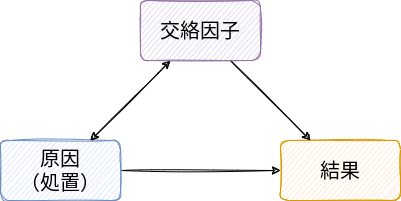
\includegraphics{figures/confounding1.drawio.png}

}

\caption{交絡のイメージ}

\end{figure}

\(\leadsto\)理想としてのRCT(および自然実験)/常に実行可能とは限らない

\(\leadsto\)その他の分析手法の開発

\hypertarget{ux7d71ux5236}{%
\section{統制}\label{ux7d71ux5236}}

RCTのポイント:原因のある(政策を受けた)集団と原因のない(政策を受けなかった)集団の性質がほとんど同じである

\(\leadsto\)事後的に同じような集団を作ればよい?

\begin{itemize}
\tightlist
\item
  性質を一致させるという意味で\textbf{統制} (control) と呼ぶ。
\end{itemize}

\hypertarget{ux30deux30c3ux30c1ux30f3ux30b0}{%
\subsection{マッチング}\label{ux30deux30c3ux30c1ux30f3ux30b0}}

\textbf{マッチング}:原因のある集団とない集団から同じような対象を取り出して比較する。\footnote{似たような発想で重み付け
  (weighting) と呼ばれる手法も用いられる。}

\begin{figure}[htpb]

{\centering 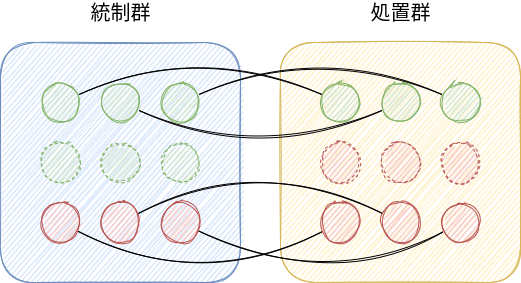
\includegraphics{figures/matching.drawio.png}

}

\caption{マッチングのイメージ}

\end{figure}

\(\leadsto\)同じような対象を常に取り出せるとは限らない。

\begin{itemize}
\tightlist
\item
  1990年に東京で生まれた生物学上の男性で大学院卒で大学教員として札幌に住んでいるビール好き?
\end{itemize}

\hypertarget{ux56deux5e30ux5206ux6790}{%
\subsection{回帰分析}\label{ux56deux5e30ux5206ux6790}}

もっぱら社会科学で広く使われているのは\textbf{回帰分析}\citep{kasuya2018}

\begin{figure}[htpb]

{\centering 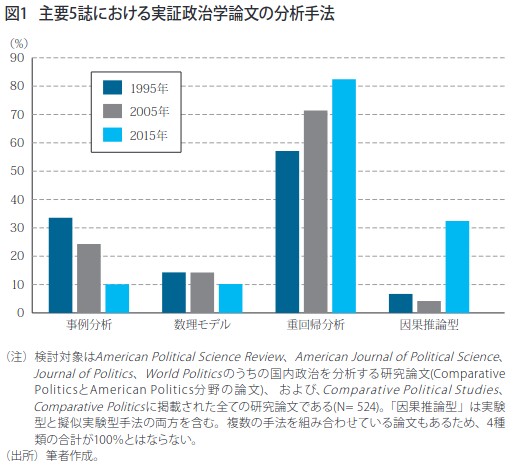
\includegraphics{figures/kasuya.png}

}

\caption{\citet{kasuya2018}}

\end{figure}

\begin{figure}[htpb]

{\centering 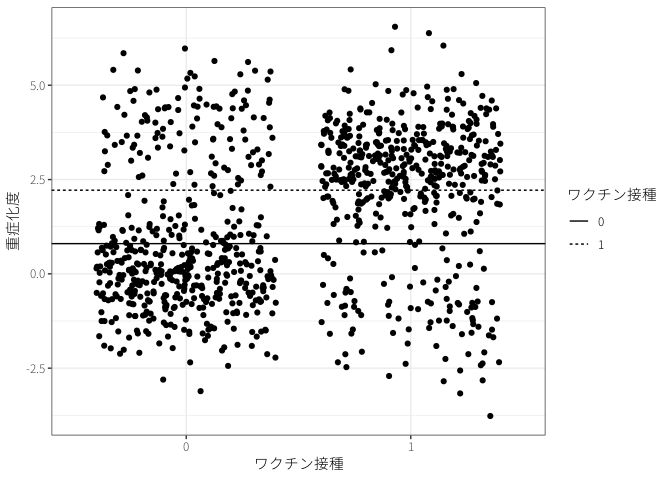
\includegraphics{causal_inference_advanced_files/figure-pdf/unnamed-chunk-2-1.png}

}

\caption{豊かさと平均寿命}

\end{figure}

\[
\textrm{平均寿命} = -9.101 + 8.405 \times \log(\textrm{一人あたりGDP})
\]

\begin{itemize}
\tightlist
\item
  毎年、一人あたりGDPも平均寿命も増加しているだけでは?
\end{itemize}

\[
\textrm{平均寿命} = -391.051 + 7.770 \times \log(\textrm{一人あたりGDP}) + 0.195 \times \textrm{年}
\]

\(\leadsto\)回帰分析に入れた特徴量の交絡は取り除くことができる。

\begin{itemize}
\tightlist
\item
  特定の年において一人あたりGDPが増えた時に平均寿命がどの程度増えるのかを示している。
\end{itemize}

マッチングも回帰分析も(後述する手法よりも)簡単に交絡を取り除ける。

\hypertarget{ux7d71ux5236ux306eux9650ux754c}{%
\subsection{統制の限界}\label{ux7d71ux5236ux306eux9650ux754c}}

マッチングも回帰分析も分析に用いた特徴量の交絡のみ取り除く。

\(\leadsto\)分析に用いていない(データとして存在しない)特徴量の交絡は取り除くことはできない。

\begin{itemize}
\tightlist
\item
  平均寿命と一人あたりGDPの交絡因子の候補は?
\end{itemize}

分析に用いた特徴量以外に交絡因子が存在しないことを証明することは不可能(悪魔の証明)

\(\leadsto\)もう少し因果関係と言いやすいような状況はないだろうか?

\begin{itemize}
\tightlist
\item
  経済学、公衆衛生学、政治学\ldots\ldots における因果推論革命、識別革命
\end{itemize}

\hypertarget{ux56deux5e30ux4e0dux9023ux7d9aux30c7ux30b6ux30a4ux30f3}{%
\section{回帰不連続デザイン}\label{ux56deux5e30ux4e0dux9023ux7d9aux30c7ux30b6ux30a4ux30f3}}

\textbf{回帰不連続デザイン} (regression discontinuity design:
RDD):ある基準を満たすかどうかで、原因の有無が分かるような状況を使ってみる。

\begin{itemize}
\tightlist
\item
  とある資格(例えば英検)を取るといい給料の仕事に就職しやすくなるのか?
\end{itemize}

\begin{figure}[htpb]

{\centering 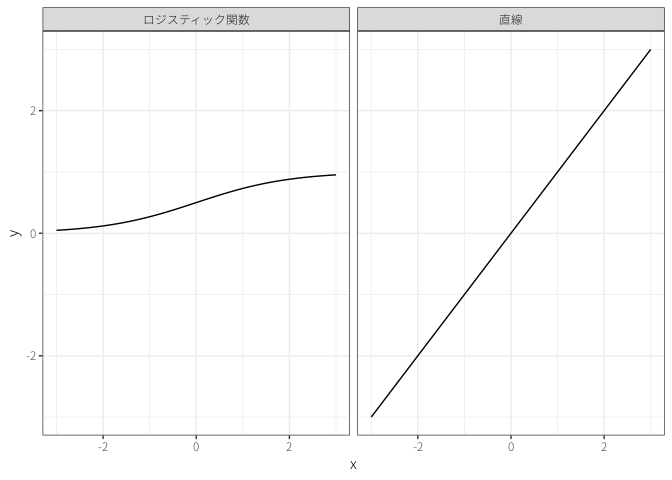
\includegraphics{causal_inference_advanced_files/figure-pdf/unnamed-chunk-3-1.png}

}

\caption{RDDのイメージ}

\end{figure}

\begin{itemize}
\tightlist
\item
  基準をぎりぎり満たした人と満たせなかった人はほとんど同じような集団かも?
\end{itemize}

\(\leadsto\)もし基準の前後で「ジャンプ」が存在していれば、それは効果と言えそう。

\begin{itemize}
\tightlist
\item
  医療費負担の引き下げは健康に資するのか?
\end{itemize}

\begin{figure}[htpb]

{\centering 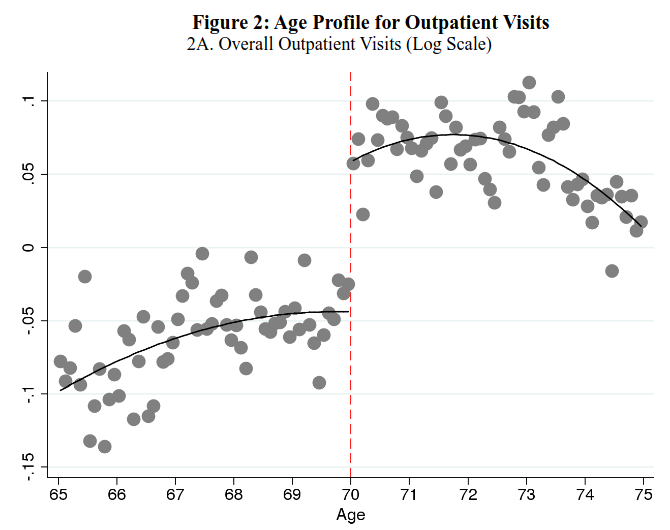
\includegraphics{figures/shigeoka1.png}

}

\caption{\citet{shigeoka2014}}

\end{figure}

\begin{figure}[htpb]

{\centering 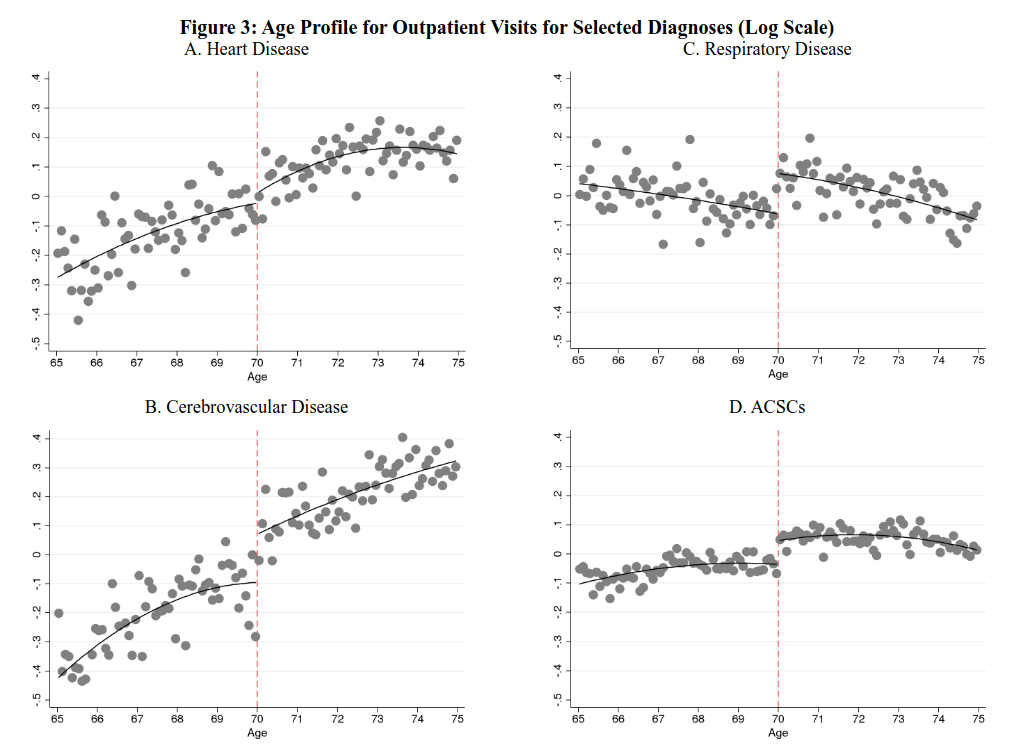
\includegraphics{figures/shigeoka2.png}

}

\caption{\citet{shigeoka2014}}

\end{figure}

\begin{itemize}
\tightlist
\item
  少人数教育は学力の向上に資するのか?
\end{itemize}

\begin{figure}[htpb]

{\centering 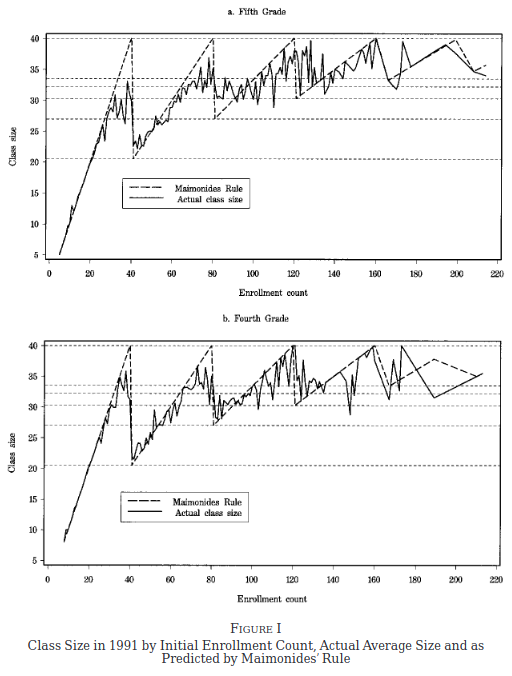
\includegraphics{figures/angrist1.png}

}

\caption{\citet{angrist1999}}

\end{figure}

\begin{figure}[htpb]

{\centering 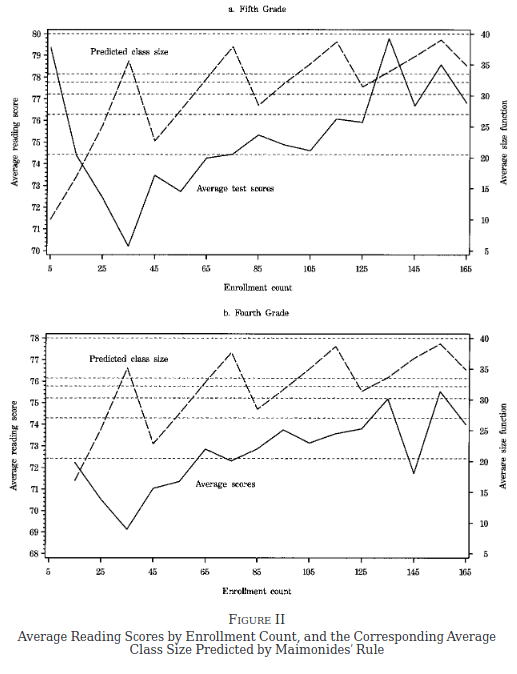
\includegraphics{figures/angrist2.png}

}

\caption{\citet{angrist1999}}

\end{figure}

\begin{itemize}
\tightlist
\item
  女性政治家(市長)は男性と異なるのか?

  \begin{itemize}
  \tightlist
  \item
    政治学でよく使われるのは、ギリギリ当選した場合と落選した場合の比較
  \end{itemize}
\end{itemize}

\begin{figure}[htpb]

{\centering 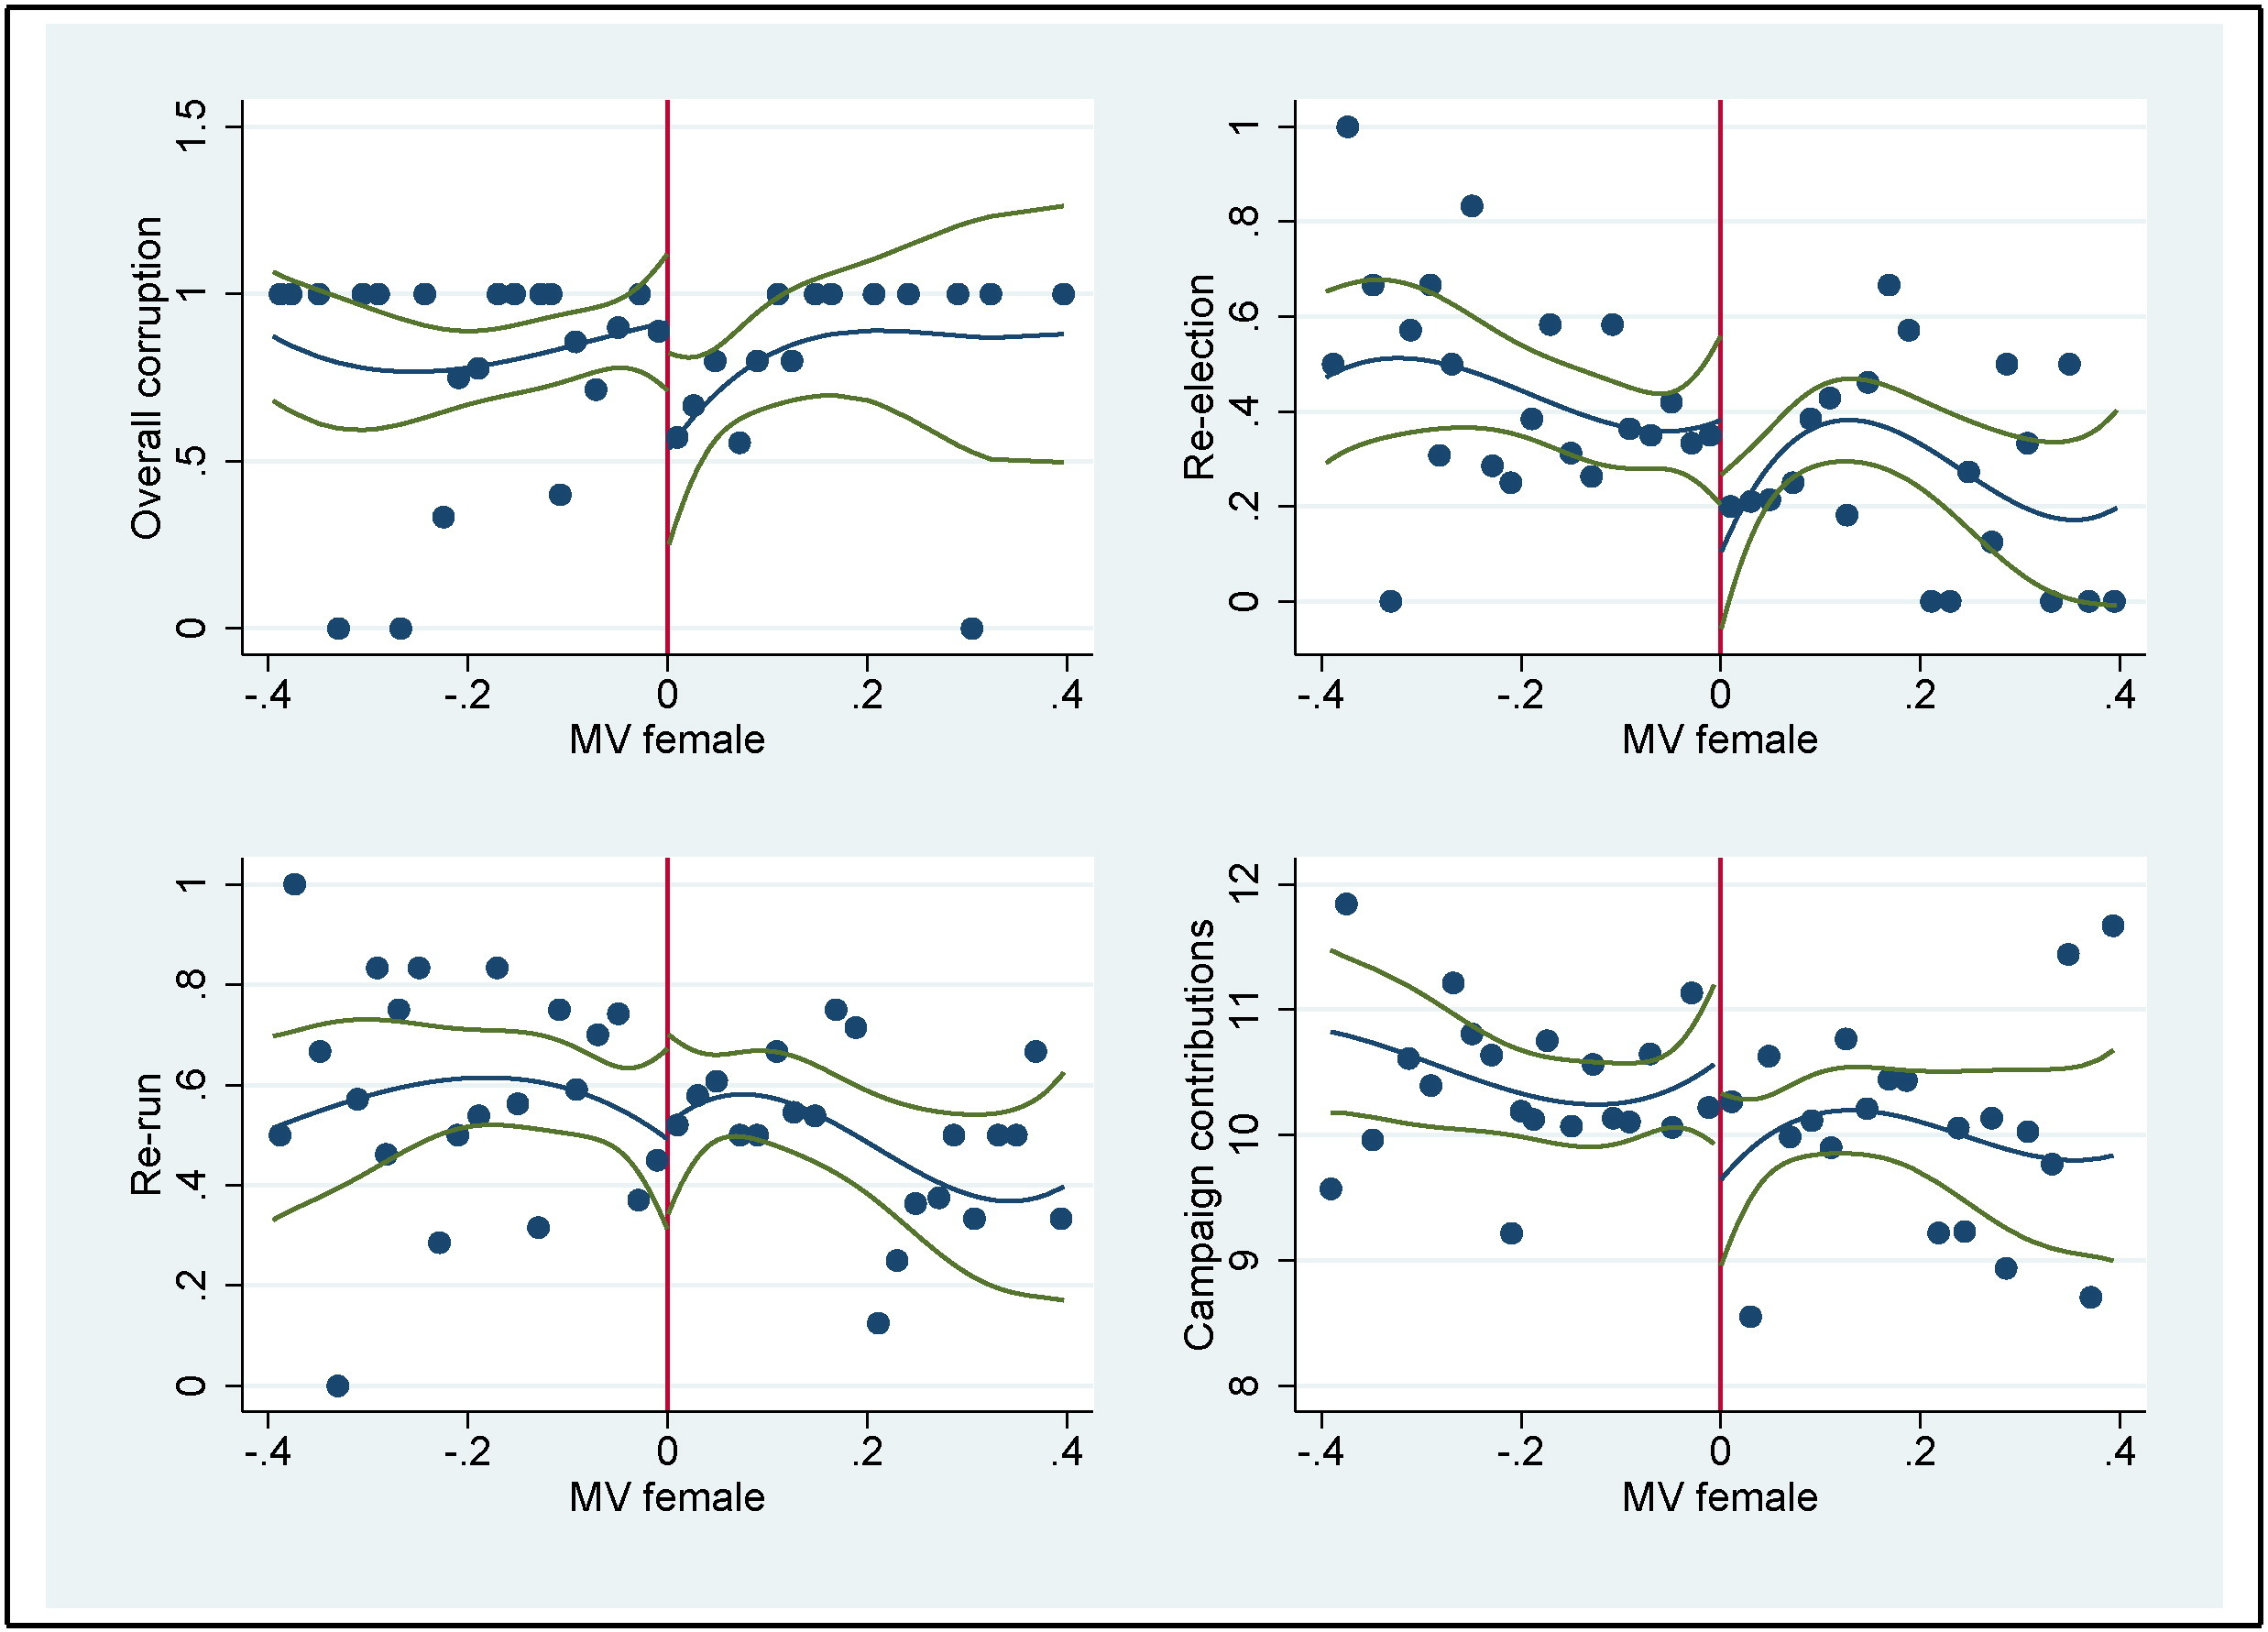
\includegraphics{figures/brollo1.jpg}

}

\caption{\citet{brollo2016}}

\end{figure}

\begin{figure}[htpb]

{\centering 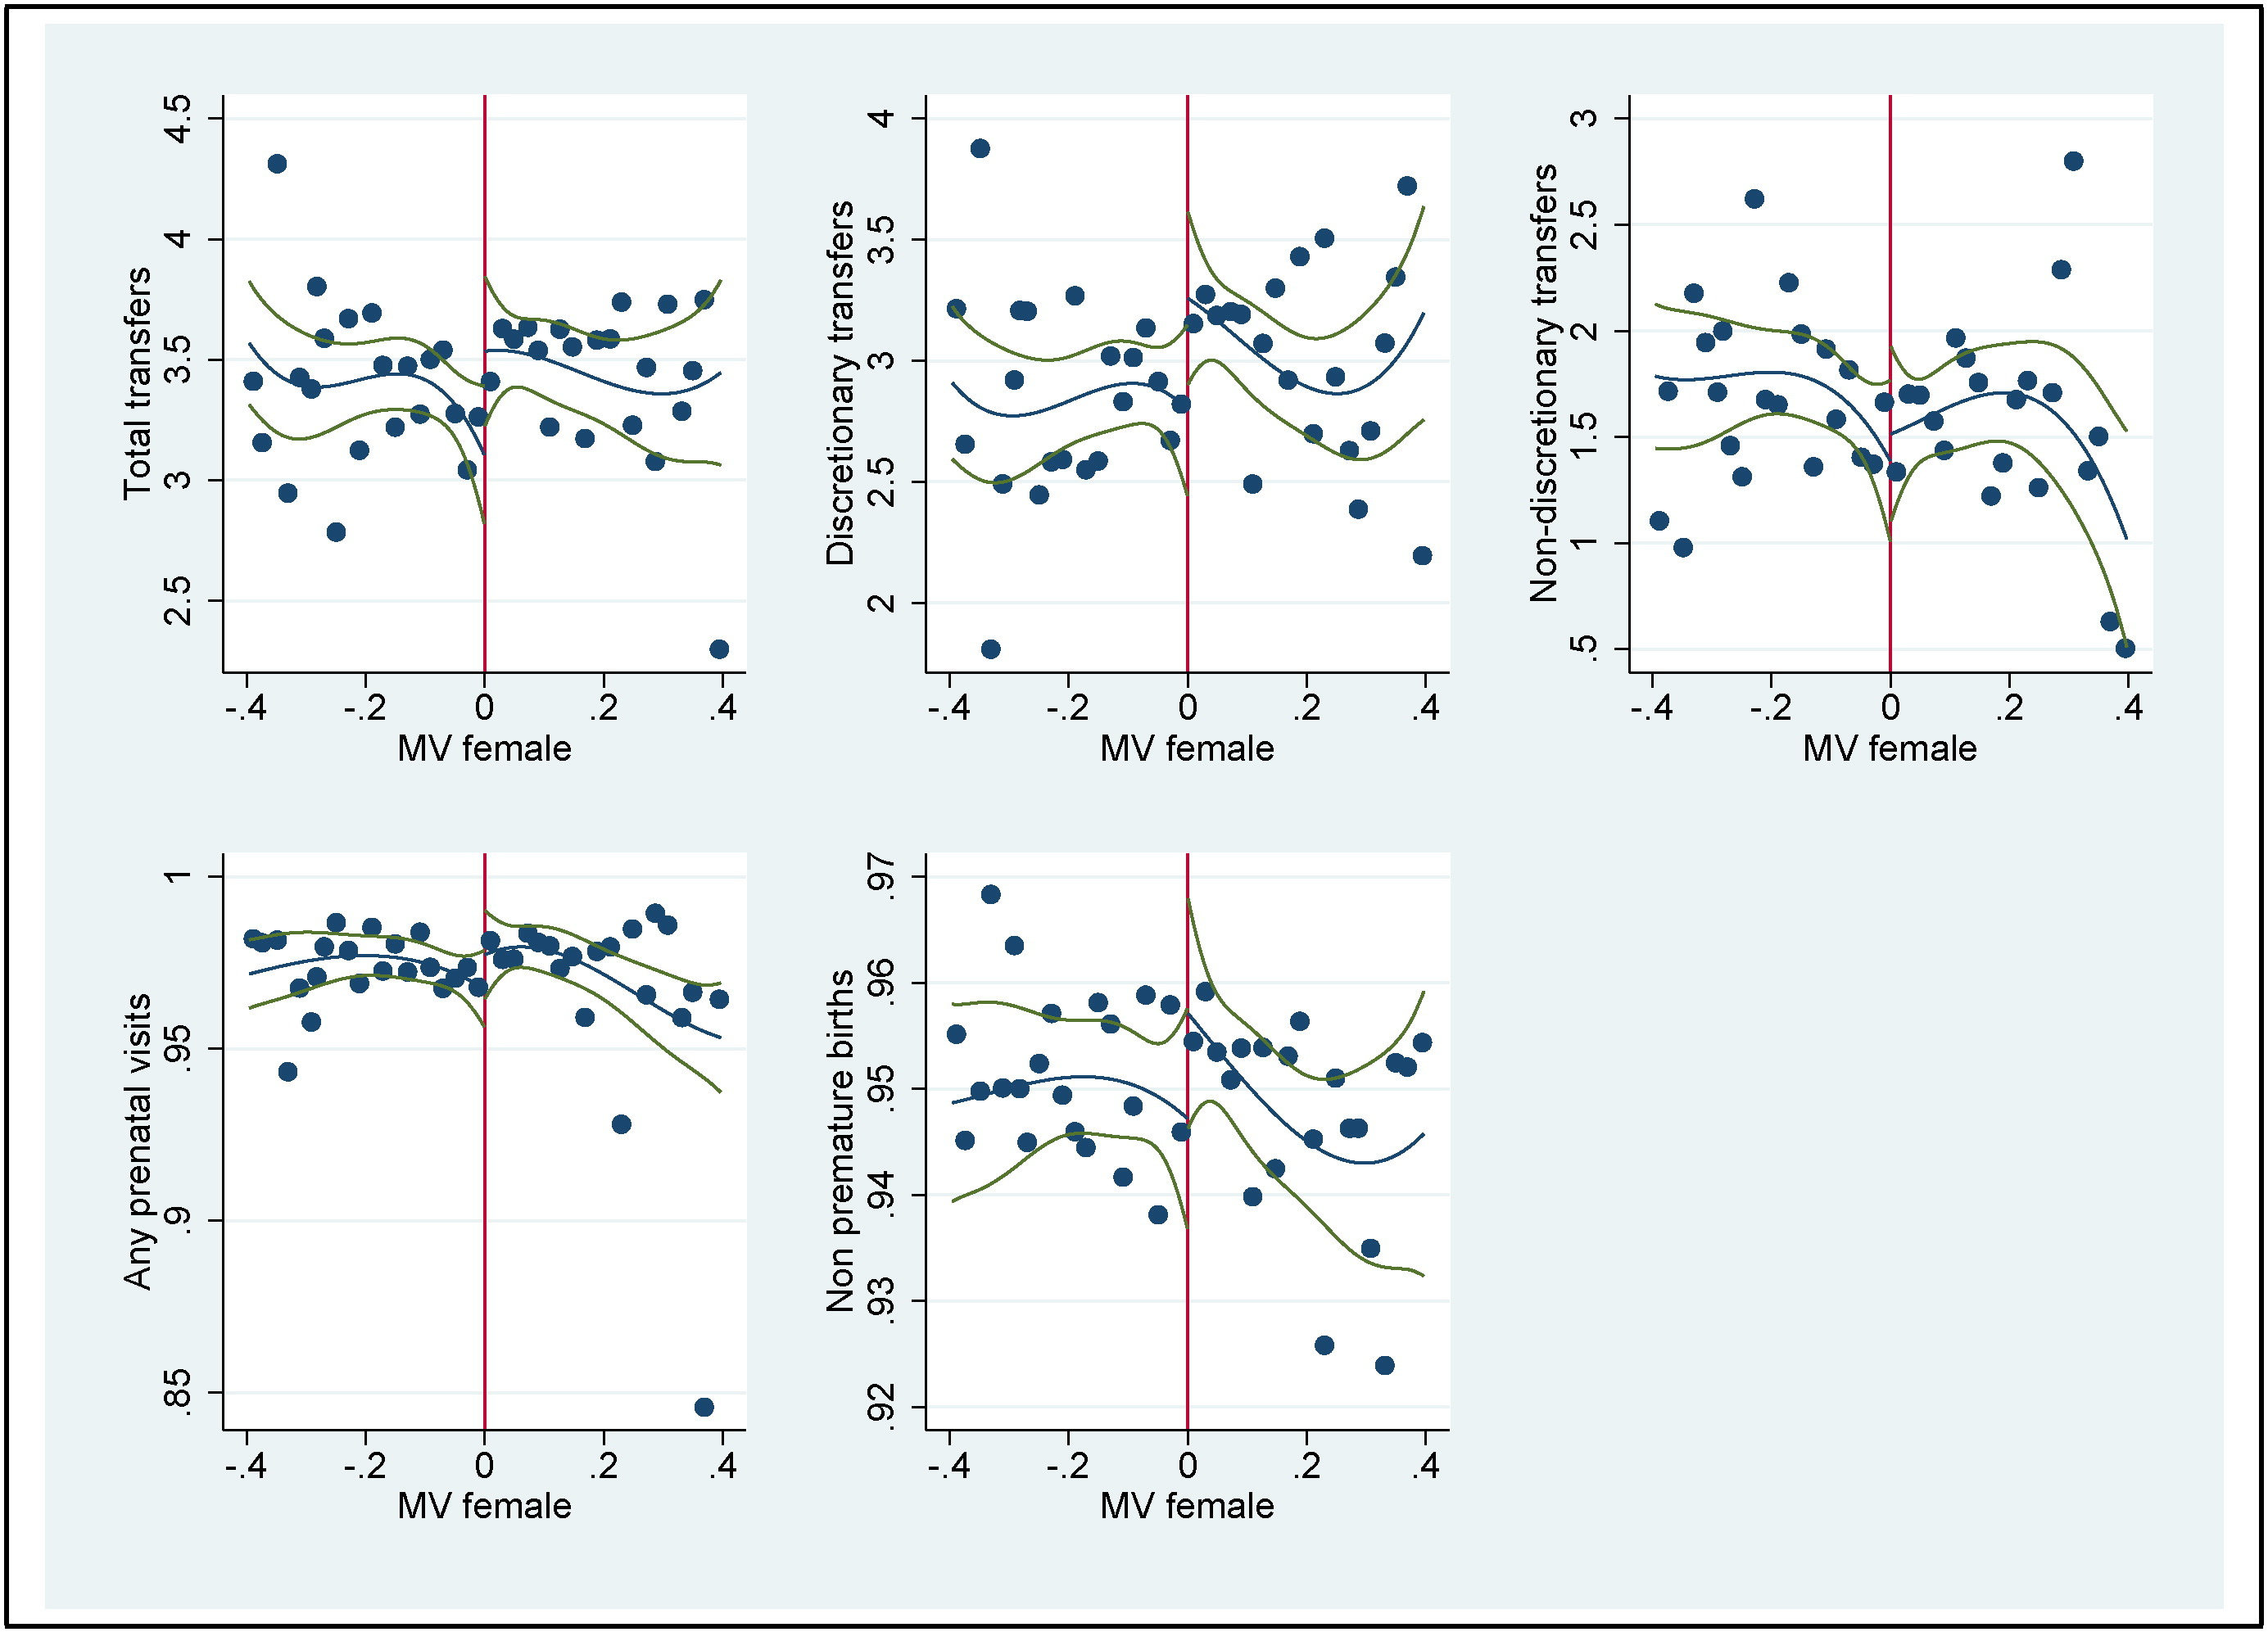
\includegraphics{figures/brollo2.jpg}

}

\caption{\citet{brollo2016}}

\end{figure}

\begin{itemize}
\tightlist
\item
  選挙広告は投票率を上げるのか?

  \begin{itemize}
  \tightlist
  \item
    地理的境界線もよく使われている。
  \end{itemize}
\end{itemize}

\begin{figure}[htpb]

{\centering 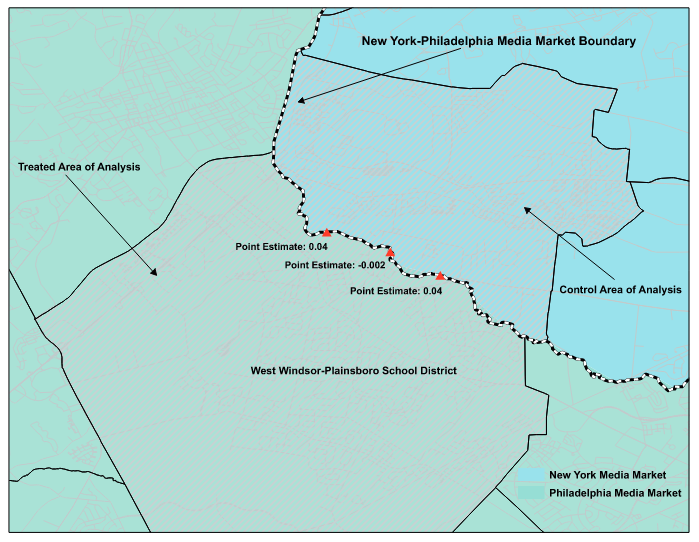
\includegraphics{figures/keele.png}

}

\caption{\citet{keele2015}}

\end{figure}

\hypertarget{ux5deeux5206ux306eux5dee}{%
\section{差分の差}\label{ux5deeux5206ux306eux5dee}}

\hypertarget{ux524dux5f8cux5373ux56e0ux679cux306eux8aa4ux8b2c}{%
\subsection{前後即因果の誤謬}\label{ux524dux5f8cux5373ux56e0ux679cux306eux8aa4ux8b2c}}

前後即因果の誤謬:結果の前に生じたものを原因とみなす誤り

\(\leadsto\)ある事象Aが起きた後に事象Bが生じたからといってAがBの原因とは言い切れない

\begin{itemize}
\tightlist
\item
  とある資格(例えば英検)を取るといい給料の仕事に就職しやすくなるのか?
\end{itemize}

\begin{figure}[htpb]

{\centering 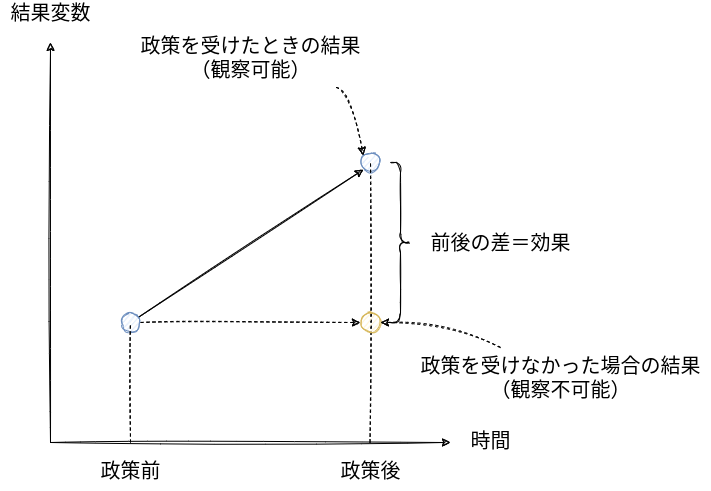
\includegraphics{figures/did1.drawio.png}

}

\caption{前後比較のイメージ}

\end{figure}

\begin{figure}[htpb]

{\centering 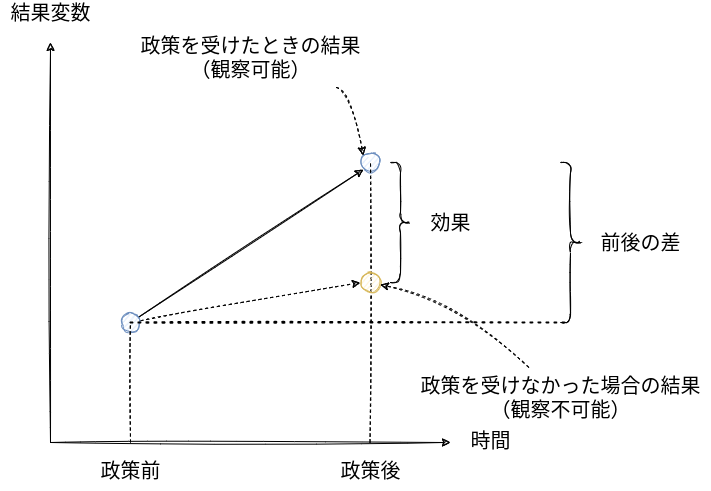
\includegraphics{figures/did2.drawio.png}

}

\caption{前後即因果の誤謬のイメージ}

\end{figure}

\begin{itemize}
\tightlist
\item
  もちろん、原因の有無で比較しても意味はない。
\end{itemize}

\begin{figure}[htpb]

{\centering 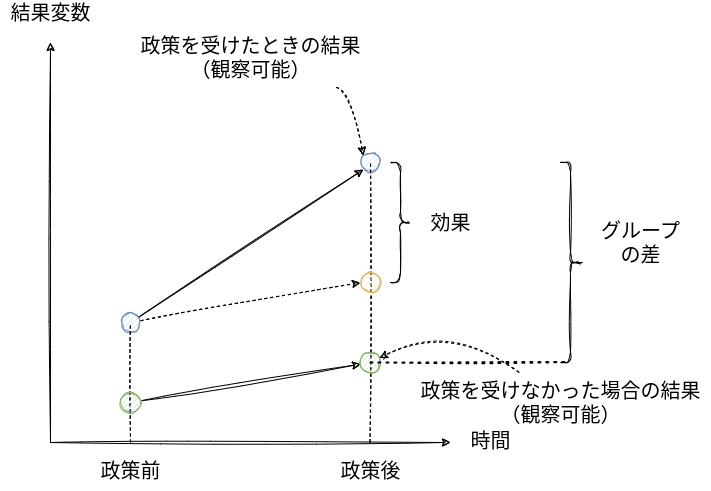
\includegraphics{figures/did3.drawio.png}

}

\caption{グループ間比較のイメージ}

\end{figure}

\hypertarget{ux5deeux5206ux306eux5dee-1}{%
\subsection{差分の差}\label{ux5deeux5206ux306eux5dee-1}}

なぜ前後比較はダメなのか?\(\leadsto\)\textbf{時間トレンド}があるから

\begin{itemize}
\tightlist
\item
  時間トレンド:原因の有無にかかわらず一定の方向へ変化する傾向
\end{itemize}

\textbf{差分の差} (difference in differences: DID)
:原因のなかったグループで時間トレンドを計算し、原因のあったグループの時間トレンドを除去する。

\begin{figure}[htpb]

{\centering 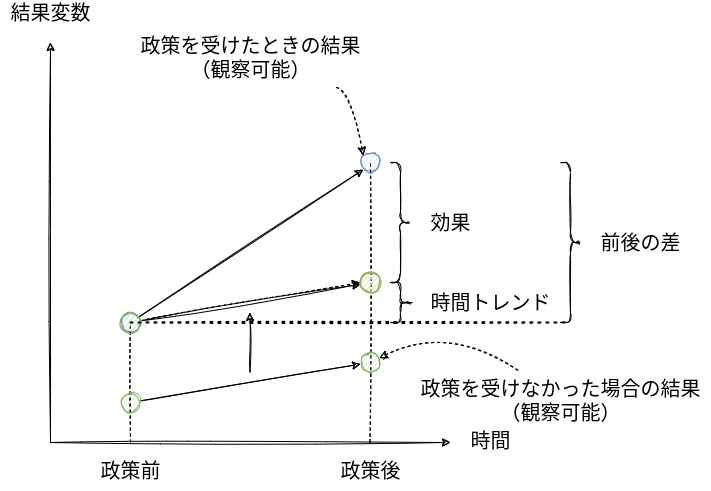
\includegraphics{figures/did4.drawio.png}

}

\caption{グループ間比較のイメージ}

\end{figure}

\begin{itemize}
\tightlist
\item
  資格を取った人の給料の増加分から資格を取らなかったひとの給料の増加分(時間トレンド)を引く。
\item
  最低賃金の上昇は雇用を減らすのか?
\end{itemize}

\begin{figure}[htpb]

{\centering 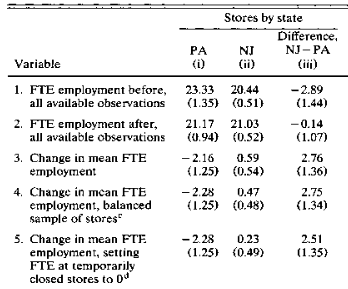
\includegraphics{figures/card1.png}

}

\caption{\citet{card1994}}

\end{figure}

\begin{itemize}
\tightlist
\item
  難民の受け入れは賃金や個用を悪化させるのか?
\end{itemize}

\begin{figure}[htpb]

{\centering 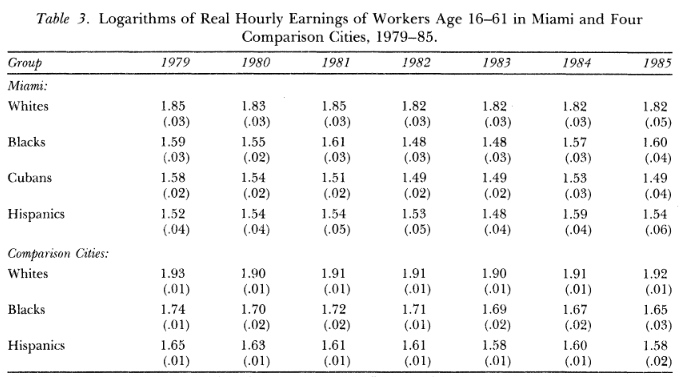
\includegraphics{figures/card2.png}

}

\caption{\citet{card1990}}

\end{figure}

\begin{figure}[htpb]

{\centering 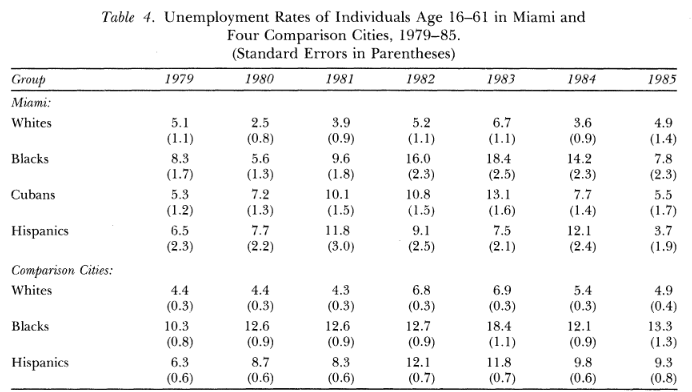
\includegraphics{figures/card3.png}

}

\caption{\citet{card1990}}

\end{figure}

\begin{itemize}
\tightlist
\item
  ヒトラーの演説はナチスへの支持を高めたのか?
\end{itemize}

\begin{figure}[htpb]

{\centering 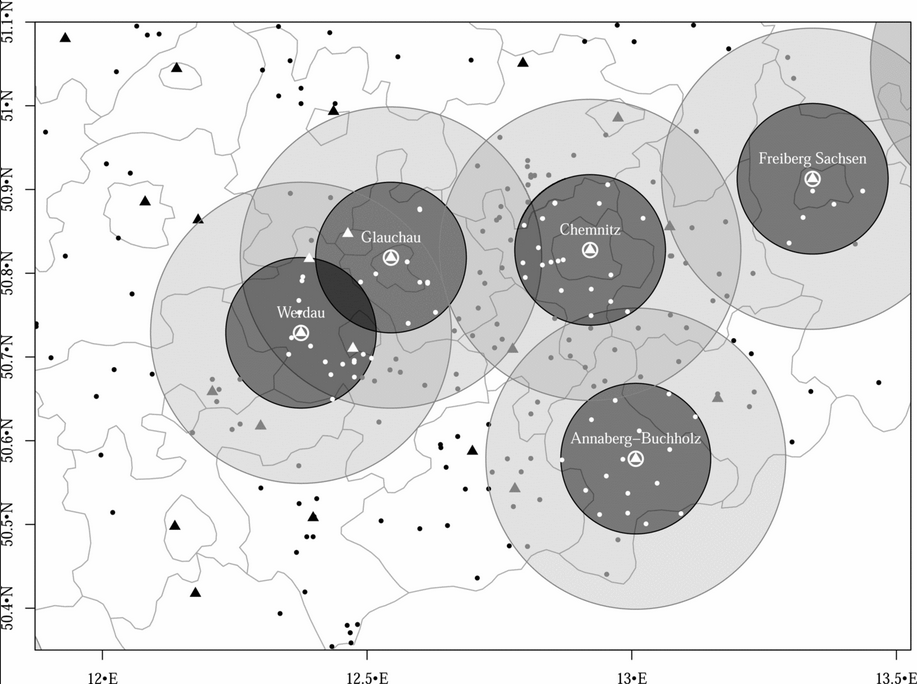
\includegraphics{figures/selb1.png}

}

\caption{\citet{selb2018}}

\end{figure}

\begin{figure}[htpb]

{\centering 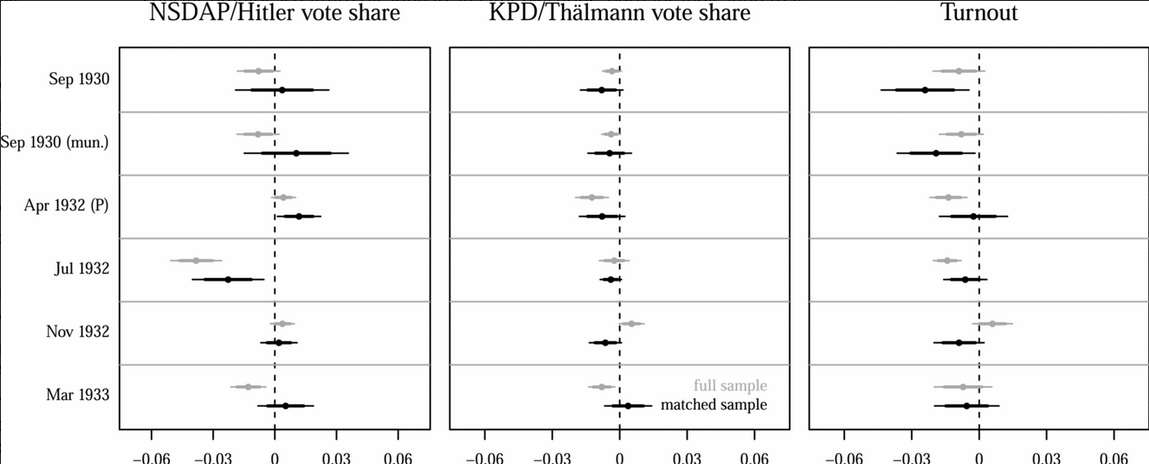
\includegraphics{figures/selb2.png}

}

\caption{\citet{selb2018}}

\end{figure}

\hypertarget{ux524dux5f8cux6bd4ux8f03ux304cux53efux80fdux306aux72b6ux6cc1}{%
\subsection{前後比較が可能な状況}\label{ux524dux5f8cux6bd4ux8f03ux304cux53efux80fdux306aux72b6ux6cc1}}

時間トレンドが無視可能な状況であれば、前後比較による効果が分かる。

\begin{enumerate}
\def\labelenumi{\arabic{enumi}.}
\tightlist
\item
  偶然(予期しない)出来事が起こった場合

  \begin{itemize}
  \tightlist
  \item
    テロリズムは政府への支持を高めるか?
  \end{itemize}
\end{enumerate}

\begin{figure}[htpb]

{\centering 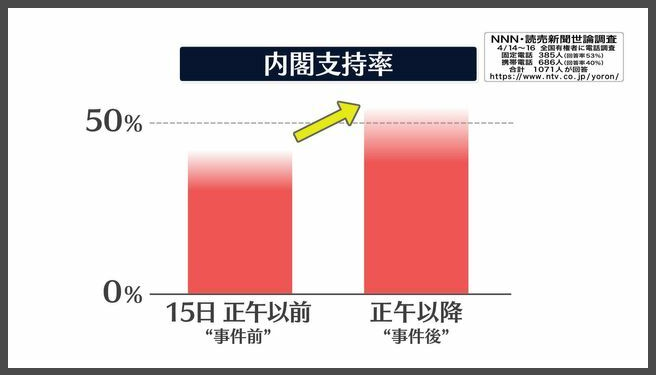
\includegraphics{figures/kishida.png}

}

\caption{\href{https://news.yahoo.co.jp/articles/b37de4c74732c92657c5d55d485852f611bc1540}{NNN読売世論調査}}

\end{figure}

\begin{enumerate}
\def\labelenumi{\arabic{enumi}.}
\setcounter{enumi}{1}
\tightlist
\item
  出来事の直前と直後(RDDの応用)を比較する場合

  \begin{itemize}
  \tightlist
  \item
    首脳の訪問は好感度を上げるのか?
  \end{itemize}
\end{enumerate}

\begin{figure}[htpb]

{\centering 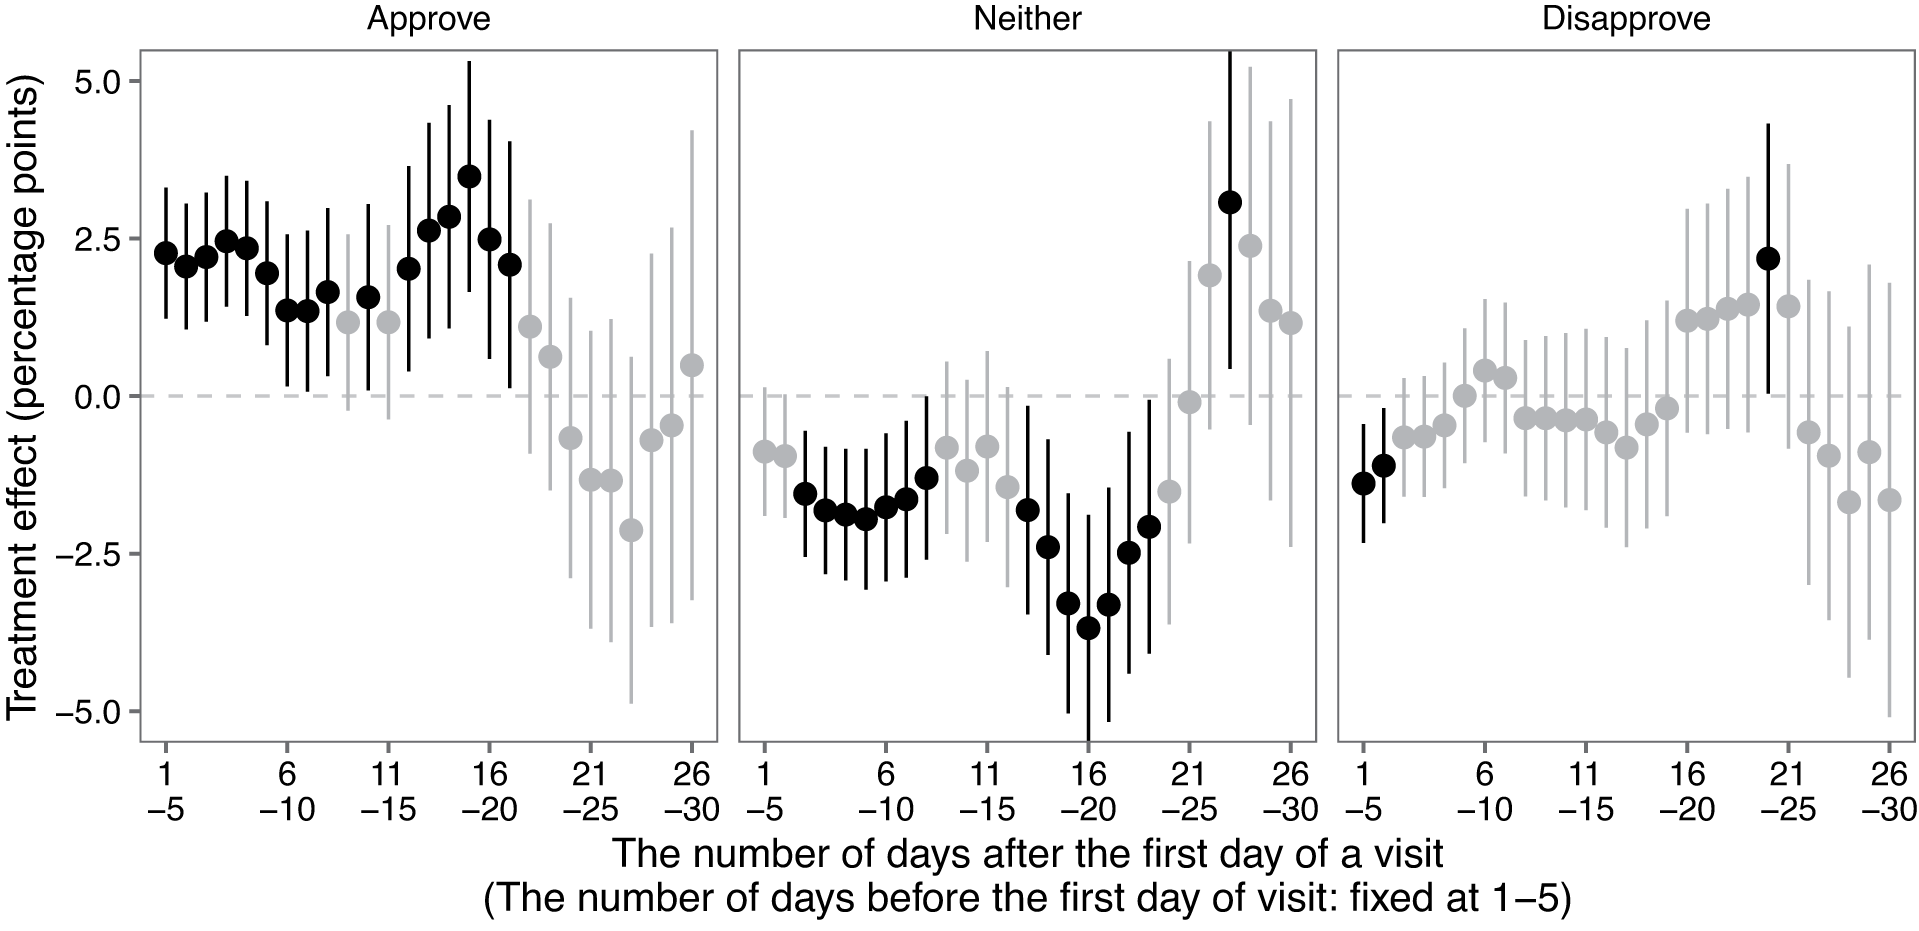
\includegraphics{figures/goldsmith.png}

}

\caption{\citet{goldsmith2021}}

\end{figure}

\hypertarget{ux5408ux6210ux7d71ux5236ux6cd5}{%
\subsection{合成統制法}\label{ux5408ux6210ux7d71ux5236ux6cd5}}

\textbf{合成統制法} (synthetic control method:
SCM):政策が起こった対象が「もし政策を行っていなかった場合」をその他の事例から合成して比較する

\begin{itemize}
\tightlist
\item
  経済の自由化は経済成長に貢献するのか?
\end{itemize}

\begin{figure}[htpb]

{\centering 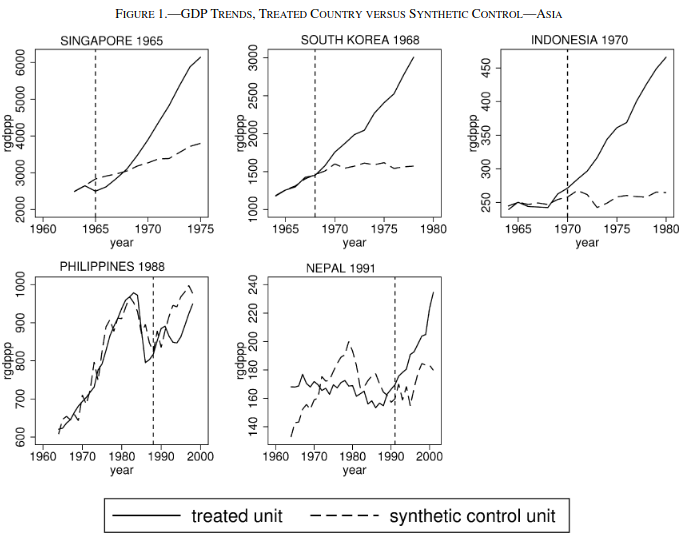
\includegraphics{figures/billmeier.png}

}

\caption{\citet{billmeier2013}}

\end{figure}

\hypertarget{ux64cdux4f5cux5909ux6570ux6cd5}{%
\section{操作変数法}\label{ux64cdux4f5cux5909ux6570ux6cd5}}

\textbf{操作変数法} (intrumental variable:
IV):原因のみに影響し、結果には直接影響しない要因(操作変数)を用いて交絡を除去する

\begin{itemize}
\tightlist
\item
  とある資格(例えば英検)を取るといい給料の仕事に就職しやすくなるのか?

  \begin{itemize}
  \tightlist
  \item
    とある資格を取るための補助をランダムに行う\(\leadsto\)その補助を受けて資格を取れるかどうかはランダム
  \end{itemize}
\end{itemize}

\begin{figure}[htpb]

{\centering 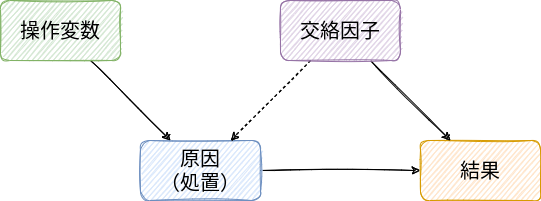
\includegraphics{figures/instrumental_variable.drawio.png}

}

\caption{操作変数のイメージ}

\end{figure}

\begin{itemize}
\tightlist
\item
  民主主義は経済成長に貢献するのか?
\end{itemize}

\begin{figure}[htpb]

{\centering 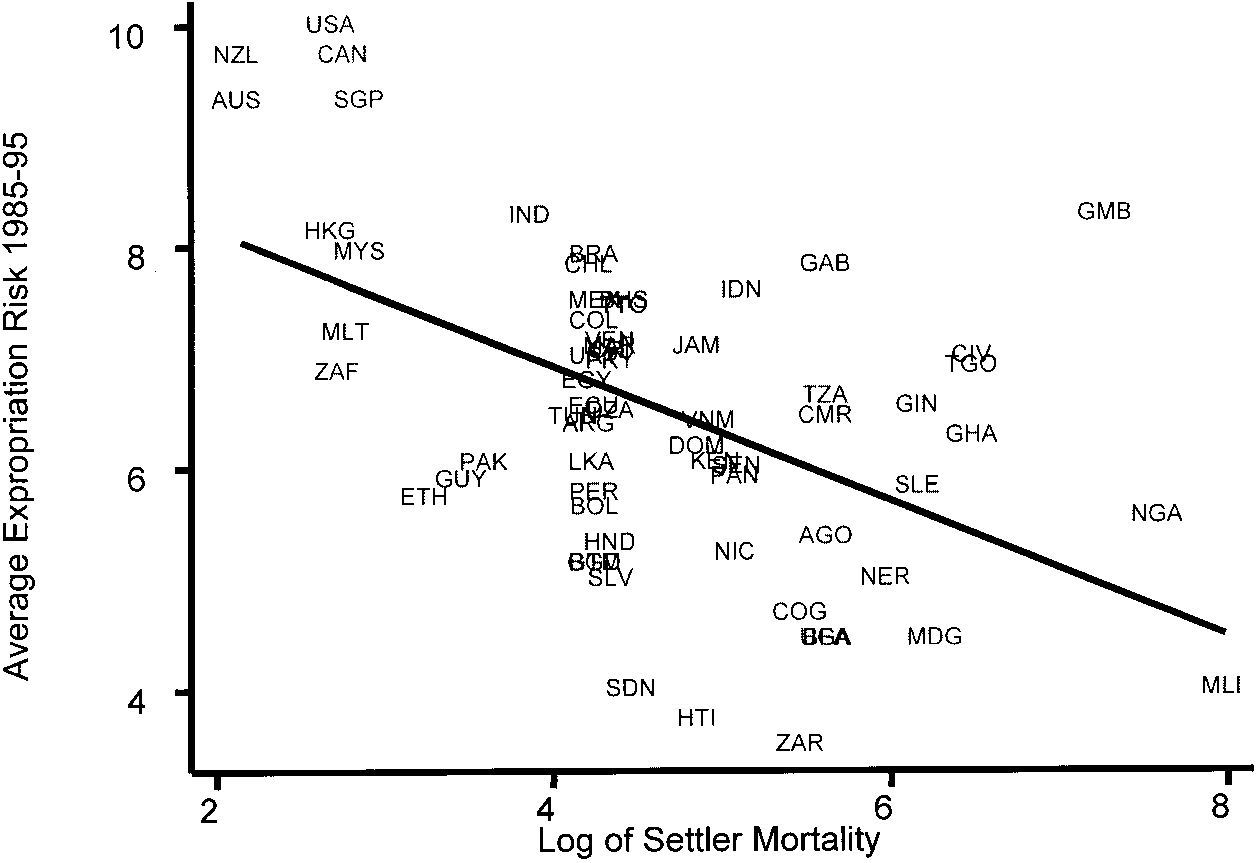
\includegraphics{figures/acemoglu1.png}

}

\caption{\citet{acemoglu2001}}

\end{figure}

\begin{figure}[htpb]

{\centering 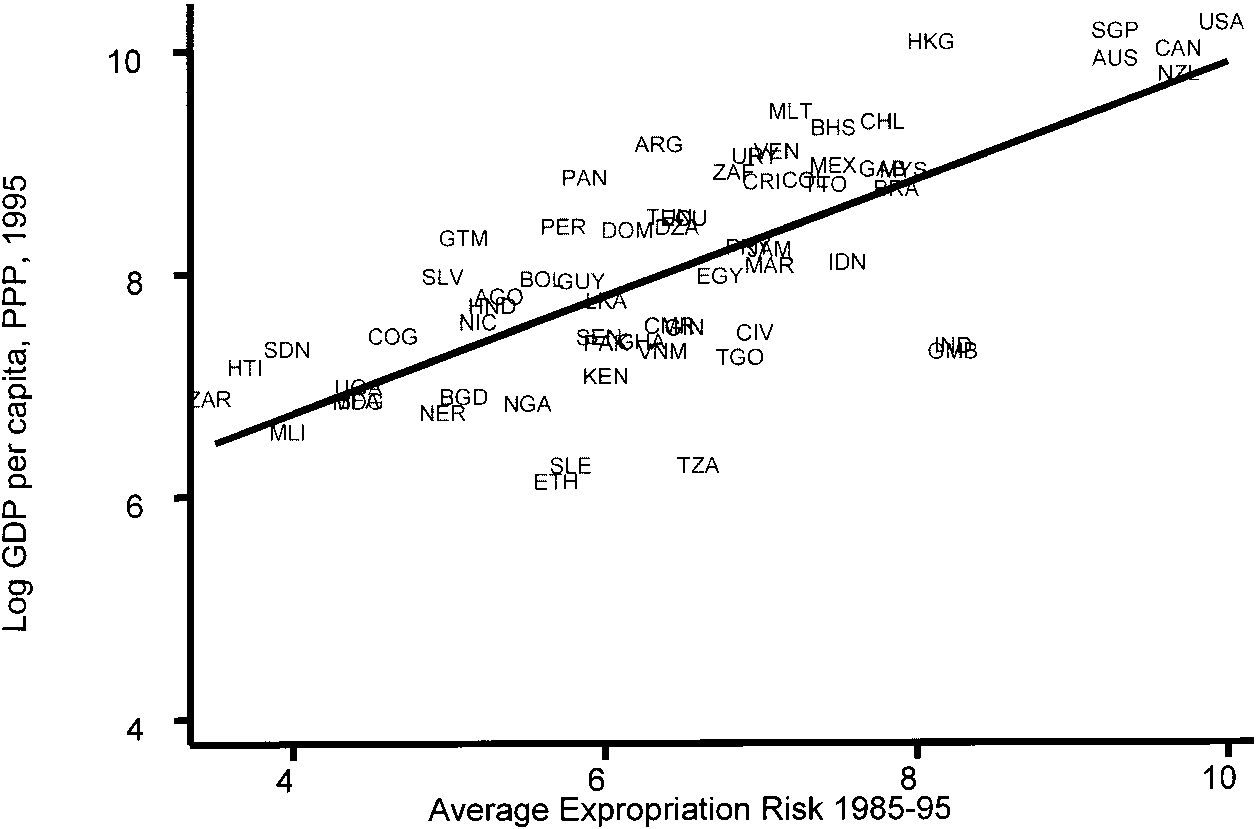
\includegraphics{figures/acemoglu2.png}

}

\caption{\citet{acemoglu2001}}

\end{figure}

\begin{itemize}
\tightlist
\item
  ナチスはプロパガンダによって支持を獲得できたのか?
\end{itemize}

\begin{figure}[htpb]

{\centering 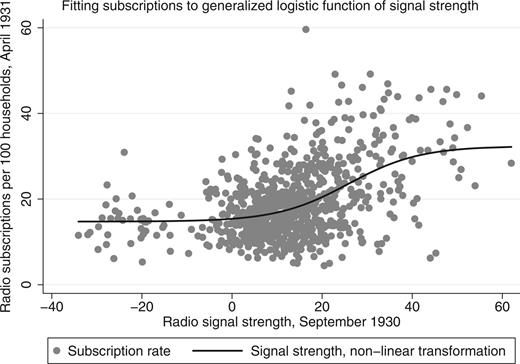
\includegraphics{figures/adena1.jpeg}

}

\caption{\citet{adena2015}}

\end{figure}

\begin{figure}[htpb]

{\centering 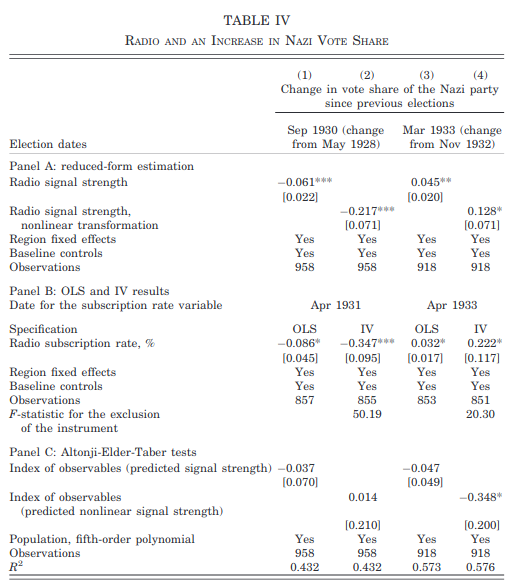
\includegraphics{figures/adena2.png}

}

\caption{\citet{adena2015}}

\end{figure}

\hypertarget{ux56e0ux679cux63a8ux8ad6ux306eux6ce8ux610fux70b9}{%
\section{因果推論の注意点}\label{ux56e0ux679cux63a8ux8ad6ux306eux6ce8ux610fux70b9}}

\hypertarget{ux30b5ux30f3ux30d7ux30ebux306eux4ee3ux8868ux6027}{%
\subsection{サンプルの代表性}\label{ux30b5ux30f3ux30d7ux30ebux306eux4ee3ux8868ux6027}}

無作為化比較試験:無作為に処置を割り当て\(\leadsto\)効果を推定

\begin{itemize}
\tightlist
\item
  \textbf{内的妥当性} (internal
  validity):手元にあるデータの中で正しく因果推論できる
\end{itemize}

無作為抽出 (random sampling):特定の集団から一部を無作為に取り出すこと

\begin{itemize}
\tightlist
\item
  \textbf{外的妥当性} (external validity)
  :分析結果が分析に用いたデータ以外にも当てはまる

  \begin{itemize}
  \tightlist
  \item
    (サンプルの)代表性:サンプルにおける属性(性別や年齢など)の割合が本当に知りたい集団と似ている。
  \item
    たとえ実験ではなくても世論調査などをする場合は無作為抽出は必要
  \end{itemize}
\end{itemize}

無作為割り当てができていても無作為抽出をしていなければ、分析結果が元々の集団に当てはまるかは分からない。

\begin{itemize}
\tightlist
\item
  もちろん、無作為抽出でも別の集団については当てはまるか分からない。
\end{itemize}

オンラインのサンプルは市民を代表しているのか?

\begin{itemize}
\tightlist
\item
  (スペインとアメリカでは)Twitterユーザーは男性、都市部の住民、政治的に極端な人が多い、あるいは多くのツイートをしている\citep{barbera2015b}
\item
  (アメリカでは)調査会社のサンプルに比べてクラウドソーシングの参加者の属性は偏っている\citep{weinberg2014}
\end{itemize}

\begin{figure}[htpb]

{\centering 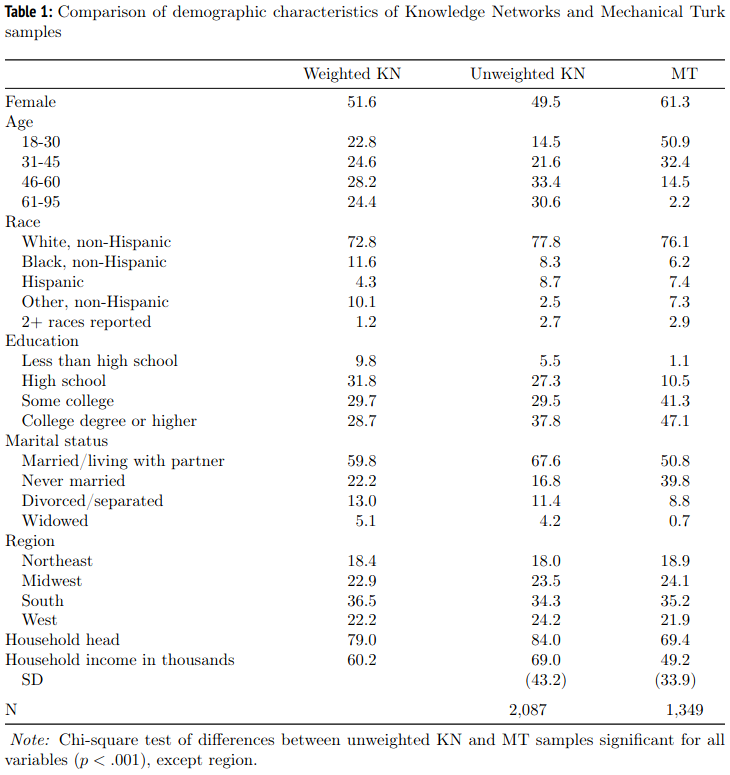
\includegraphics{figures/weinberg.png}

}

\caption{\citet{weinberg2014}}

\end{figure}

\begin{itemize}
\tightlist
\item
  ただし、RCTの結果はどちらでも同じような傾向を持つ\citep{weinberg2014}
\end{itemize}

\hypertarget{ux4e0dux5747ux4e00ux52b9ux679c}{%
\subsection{不均一効果}\label{ux4e0dux5747ux4e00ux52b9ux679c}}

政策の効果はあらゆる集団に対して同じとは限らない。

\begin{itemize}
\tightlist
\item
  年齢や性別、学歴、経済状況\ldots\ldots などによって効果は変わりうる。
\end{itemize}

\begin{figure}[htpb]

{\centering 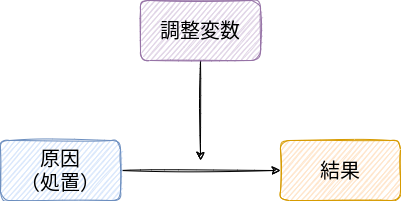
\includegraphics{figures/interaction.drawio.png}

}

\caption{条件付き効果}

\end{figure}

\(\leadsto\)条件ごとに集団を分割して効果を推定する。

\hypertarget{ux4e00ux822cux5747ux8861ux52b9ux679c}{%
\subsection{一般均衡効果}\label{ux4e00ux822cux5747ux8861ux52b9ux679c}}

RCTでは集団全体から一部を取り出して、政策の有無を決定する。

\(\leadsto\)実際に政策を受けるのは全体から見るとごく一部

政策として集団全体に実施した場合は、RCT通りの結果にならないかもしれない。

\(\leadsto\)集団全体における効果(一般均衡効果)が生じる。

\begin{itemize}
\tightlist
\item
  職業訓練や教育が賃金を上げるとしても、全員がプログラムを受けるとその効果は相殺?
\item
  少人数にSNSをやらせても意味はない?
\end{itemize}

\begin{figure}[htpb]

{\centering 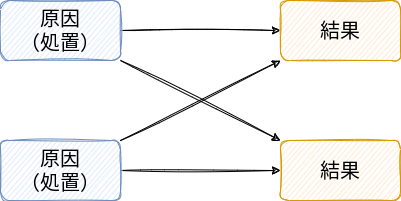
\includegraphics{figures/diffusion.drawio.png}

}

\caption{効果の波及}

\end{figure}

効果が波及する場合:RCTは適切に政策の効果を推定できない。

\hypertarget{ux5b9fux8a3cux5206ux6790ux3078ux306eux793aux5506}{%
\section{実証分析への示唆}\label{ux5b9fux8a3cux5206ux6790ux3078ux306eux793aux5506}}

実際に因果推論しなくても、実証分析をする上で重要な点はある(と信じている)

\hypertarget{ux8a08ux91cfux5206ux6790}{%
\subsection{計量分析}\label{ux8a08ux91cfux5206ux6790}}

とりあえず実際のデータに触れてみるという姿勢は大事

関係分野のデータ分析の研究に触れてみるのも大事

\begin{itemize}
\tightlist
\item
  案外、反直観的な(予想と異なる)結果が得られることはある。
\item
  政治学や経済学の一般向けの本\citep{banerjee2020, kitamura2020}
\end{itemize}

データ分析だからといって鵜呑みにするのも危険

\begin{itemize}
\tightlist
\item
  どのようなデータと手法を用いているのかを確認
\item
  「データの読み方」を学ぶ\citep{sugawara2022, ogiwara2023, tsutsui2023}
\end{itemize}

\hypertarget{ux4e8bux4f8bux5206ux6790}{%
\subsection{事例分析}\label{ux4e8bux4f8bux5206ux6790}}

事例分析をする際にも効果を示す際には注意が必要\citep{kume2013, ito2022}

\begin{itemize}
\tightlist
\item
  差異法:同じような事例だが、原因の有無が異なるような事例を比較する

  \begin{itemize}
  \tightlist
  \item
    理想としては原因がランダムに生じている状況
  \item
    原因が生じた直前と直後の比較
  \item
    時間トレンドの確認
  \end{itemize}
\item
  一致法:異なる事例だが、原因と結果が生じている事例を比較する

  \begin{itemize}
  \tightlist
  \item
    有力な原因を提案できるが、因果関係・効果を主張するのは難しい
  \end{itemize}
\item
  反実仮想:仮に原因がなかったらどうなっていたのかを明らかにして、原因であることを説得する
\item
  過程追跡:原因から結果での出来事の連鎖を辿って、因果関係・プロセスを示す
\item
  逸脱事例:通説では説明できない事例を提示して、通説を修正する
\end{itemize}


  \bibliography{references.bib}


\end{document}
